\documentclass[times, utf8, diplomski, english]{fer}
\usepackage{booktabs}
\usepackage[hidelinks]{hyperref}
\usepackage{footnote}
\usepackage{graphicx}

\usepackage{listings}
\usepackage{protobuf/lang}  % include language definition for protobuf
\usepackage{protobuf/style} % include custom style for proto declarations.

\DeclareMathOperator*{\argmin}{\arg\!\min}
\DeclareMathOperator*{\argmax}{\arg\!\max}
\graphicspath{ {./figures/} }

\begin{document}

\thesisnumber{1572}
\title{ End-to-End Deep Learning Model for Base Calling of MinION Nanopore Reads}
\author{Neven Miculinić}
\maketitle
 
\izvornik

\zahvala{I would like to thank my mentor, Mile Šikić, for his patient guidance, encouragement
    and advice provided over the years.
    
I would also like to thank my family and friends for their
    continuous support.
    
In the end, honorable mentions go to Marko Ratković for his help with this thesis.	
}

\tableofcontents
\listoffigures
\listoftables

%%%%%%%%%%%%%%%%%%%%%%%%%%%%%%%%%%%%%%%%%
% Chapter Introduction
%%%%%%%%%%%%%%%%%%%%%%%%%%%%%%%%%%%%%%%%%
\chapter{Introduction}
\label{chap:Introduction}
In recent years,  deep learning methods significantly improved the state-of-the-art in multiple domains such as computer vision, speech recognition, and natural language processing \cite{LeCun:1998:CNI:303568.303704}\cite{NIPS2012_4824}. 
In this thesis, we present application of deep learning in the field of  Bioinformatics for analysis of DNA sequencing data. 

DNA is a molecule that makes up the genetic material of a cell, and it is responsible for carrying the information needed for survival, growth, and reproduction of an organism. 
DNA is a long polymer of simple blocks called nucleotides connected together forming two spiraling strands to a structure called a double helix.  Possible nucleotide bases of a DNA strand are adenine, cytosine, guanine, thymine usually represented with letters A, C, G, and T. The order of these bases is what defines genetic code.

DNA sequencing is the process of determining this sequence of nucleotides. Originally sequencing was an expensive process, but during the last couple of decades, the price of sequencing has drastically decreased.  A significant breakthrough occurred in May 2015 with the release of MinION sequencer by Oxford Nanopore making DNA sequencing inexpensive and more available, even for small research teams. 

Base calling is a process assigning sequence of nucleotides (letters) to the raw data generated by the sequencing device. Simply put, it is a process of decoding the output from the sequencer.
\section{Objectives}
The objective of this thesis is try out novel approach in basecalling the raw sequence. We had good results with earlier R9 chemisty \citep{miculinic2017mincall} and we're experimenting with new approaches.
\section{Organization}

%%%%%%%%%%%%%%%%%%%%%%%%%%%%%%%%%%%%%%%%%
% Chapter Background
%%%%%%%%%%%%%%%%%%%%%%%%%%%%%%%%%%%%%%%%%

\chapter{Background}
\label{chap:background}
Due to technical constraints, it's infeasible  to sequence whole DNA in single strand. 
Every sequencing technology to date have an upper limit how big strand can it precisely sequence.
This limit is considerably smaller than size of genome.
For example E.Coli has ~4.5 million base pairs in its DNA, while Sanger's sequencing maximum output is around 1000 base pairs max.
To make DNA basecalling feasible technique called shotgun sequencing was invented. 
The strand is cloned number of times, then via chemical  agent broken down into smaller fragments of appropriate length. 
Sequenced fragments are called reads.

Genome assembly is the process of reconstructing the original genome from reads and usually starts with finding overlaps between reads.
The quality of reconstruction heavily depends on the length and the quality (accuracy) of the reads produced by the sequencer. 

If we have reference sequence we usually align the reads on the reference to aid us into genome assembly. Otherwise we have to use many de novo assembly techniques.

The right analogy would be building a puzzle. Since we cannot scan the whole puzzle because our camera is too small or imprecise, we are scanning pieces of the whole picture. Puzzle pieces would represent fragments in this analogy. If we have a map, even a rough one, it shall aids us into assemblying those puzzle pieces into complete pictures. Otherwise we're fiddling in the dark and using de novo assembly techniques.

Figure \ref{fg:sequencing} depicts process of sequencing visually.

\begin{figure}[!ht]
    \begin{center}
        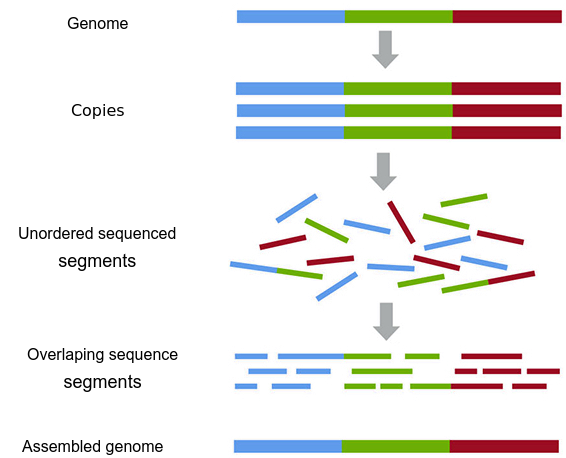
\includegraphics[width=0.6\textwidth]{shotgun-sequencing}
        \caption{Depiction of the sequencing process. Taken from \citep{mratkovic} with authors permission}
        \label{fg:sequencing}
    \end{center}
\end{figure}


Development of sequencing started with work of Frederick Sanger \cite{mile} \cite{Pettersson2009}. In 1977, he developed the first sequencing method which allowed 
read lengths up to 1000 bases with very high accuracy (99.9\%) at the cost of 1\$ per 1000 bases.
Second generation sequencing (IAN Torrent and Illumina devices) reduced the price of sequencing while maintaining high accuracy. Mayor disadvantage of these devices is read length of only a few hundred base pairs. Short reads make resolving repetitive regions practically impossible.

The need for technology able of producing longer reads led to the development of so-called third generation sequencing technologies.
PacBio developed sequencing method that allowed read lengths up to several thousand bases but at the cost of smaller accuracy. Error Rates of PacBio devices are \textasciitilde10-15\%. 

Cost makes the biggest obstacle stopping widespread genome sequencing. The release of, previously mentioned, MinION sequencer made sequencing less expensive and even portable.

\section{Oxford Nanopore MinION}

The MinION device by Oxford Nanopore Technologies is the first portable DNA sequencing device. Its small weight, low cost, and long read length combined with decent accuracy yield promising results in various applications including full human genome assembly \cite{human_seq} what could potentially lead to personalized genomic medicine.

\subsection{Technology}
As its name says, nanoscaled pores are used to sequence DNA. An electrical potential is applied over a membrane in which a  pore is inserted. 
As the DNA passes through the pore, the sensor detects changes in ionic current caused by different nucleotides present in the pore. Figure \ref{fg:nanopore} shows the change of ionic current as DNA strain is pulled through a nanopore.

\begin{figure}[!ht]
    \begin{center}
        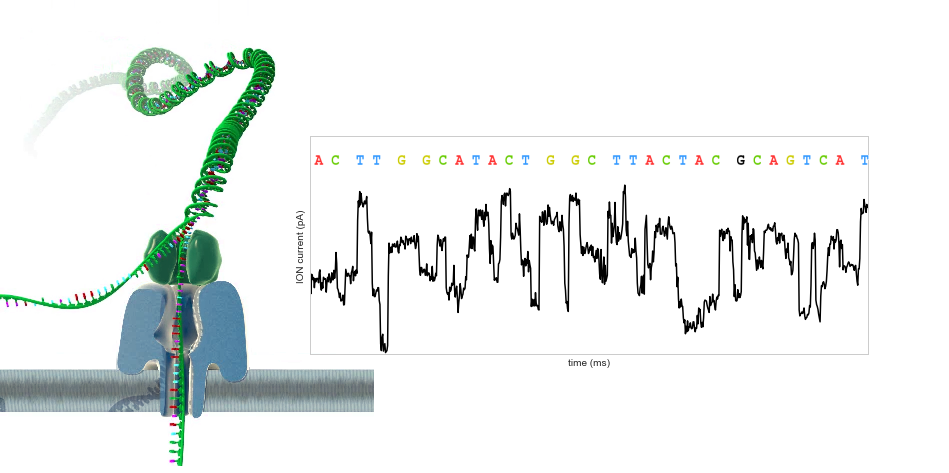
\includegraphics[width=0.7\textwidth]{nanopore}
        
        \caption[DNA strain being pulled through a nanopore]{DNA strain being pulled through a nanopore \protect\footnotemark}
        \label{fg:nanopore}
    \end{center}
\end{figure}
\footnotetext{Figure adapted from https://nanoporetech.com/how-it-works}


Official software called MinKNOW outputs sequencing data in FAST5 (a variant of the HDF5 standard) file format. It is a hierarchical file format with data arranged in a tree-structure of groups. Metadata are stored in group and dataset attributes. The same file format is during used different stages of analyses and groups, datasets and attributes are added incrementally. Figure \ref{fg:fast5} shows raw signal being present in the FAST5 file.
\begin{figure}[!ht]
    \begin{center}
        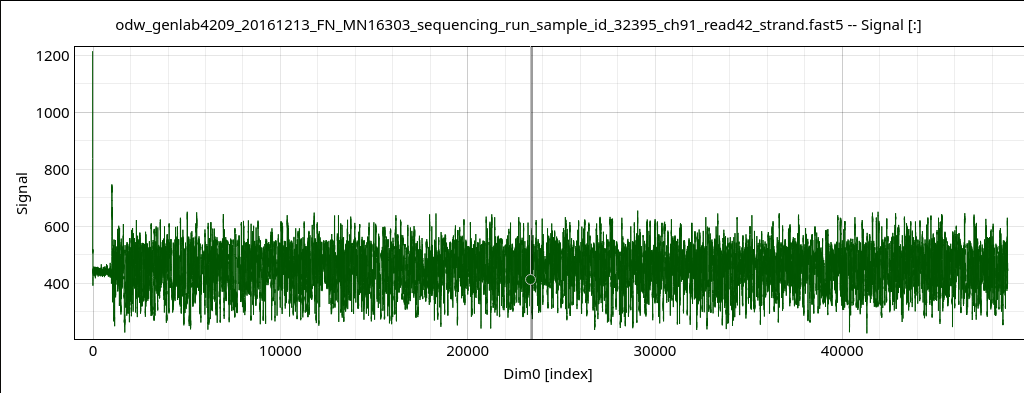
\includegraphics[width=0.6\textwidth]{fast5_sample}
        \caption[Structure of FAST5 file and raw signal plot show in \textit{HDFView}]{Structure of FAST5 file and raw signal line plot show in \textit{HDFView} \protect\footnotemark}
        \label{fg:fast5}
    \end{center}
\end{figure}
\footnotetext{https://support.hdfgroup.org/products/java/hdfview/}

Minion offers the possibility of sequencing one or both strands of DNA. Sequencing both strands and combining information results in reads of higher quality. Those reads are called 2D (two-dimensional) reads. Otherwise, if the only single strand is sequenced 1D (one-dimensional) reads are produced.

MinION devices can produce long reads, usually tens of thousand base pairs (with reported reads lengths of 100 thousand \cite{loman1-100k} and even recently above 800 thousand base pairs \cite{loman2-800k}), but with high sequencing error than older generations of sequencing technologies.
Switch from older R7.3 to  R9 chemistry in 2016 increased accuracy of produced data. With this change, the accuracy of 1D data increased from 70\% to 85\% and the accuracy of 2D reads from 88\% to 94\% \cite{nanopore_video}.  This increase of accuracy makes 1D reads usable for analysis with benefits over 2D reads being faster sample preparation and faster sequencing. Developed tool in this thesis focuses on base calling 1D reads.


  
\section{Existing basecallers}

\subsection{Official}
Oxford Nanopore has, with the R9 version of the platform, introduced a variety of base calling options. Some of those are production ready and some experimental. The majority of information regarding differences, specifications and similar is only available through Nanoporetech Community \footnote{https://community.nanoporetech.com/}.


\textit{Metrichor} is an Oxford Nanopore company that offers cloud-based platform \textit{EPI2ME} for analysis of nanopore data. 
Initially, base calling was only available by uploading data to the platform - that being the reason why this basecaller is often called Metrichor even though it is a name of the company.

The older version of Metrichor relied on \textit{hidden Markov models} (HMM) to find the biological sequence corresponding to the signal. Preprocess included segmentation of the signal into smaller chunks called events defined by start location of the chunk, length, mean value and variance of the signal in the chunk. Metrichor than assumed that each event usually corresponds to a context of 6 bases being present in the pore and that the context is typically shifted by one base in each step. 
The states of HMM are modeled as a context present in the pore and transition correspond to change of bases in the pore. During the transition from one state to another, an event is emitted. Base calling is performed using the Viterbi algorithm which determines the most likely sequence of states for the observed sequence of events. This approach showed poor results when calling long homopolymer stretches as the context in the pore remains the same \cite{homopolymers}\cite{homopolimeri_analiza}.

With the release of R9 chemistry, this model was replaced by a more accurate recurrent neural network (RNN) implementation. Currently, Oxford Nanopore offers several RNN-based local basecaller versions under different names: Albacore, Nanonet and basecaller integrated into MinKNOW \cite{ont-basecallers}.   

\textit{Albacore} is basecaller by Oxford Nanopore Technologies ready for production and actively supported.
It is available to the Nanopore Community served as a binary. The source code of Albacore was not provided and is only available through the ONT Developer Channel. Tool supports only R9.4 and future R9.5 version of the chemistry.

\textit{Nanonet}\footnote{\url{https://github.com/nanoporetech/nanonet/}} uses the same neural network that is used in Albacore but it is continually under development and does contain features such as error handling or logging needed for production use. It uses \textit{CURRENNT} library for running neural networks. It supportes basecalling of both R9 and R9.4 chemistry versions.


\textit{Scrappie}\footnote{\url{https://github.com/nanoporetech/scrappie}} is another basecaller by Oxford Nanopore Technologies. Similar to Nanonet, it is the platform for ongoing development. Scrappie is reported to be the first basecaller  that specifically address homopolymer base calling. It became publicly available just recently in June, 2017 and supports R9.4 and future R9.5 data.

\pagebreak
\subsection{Third-party basecallers}

\textit{Nanocall} \cite{David046086} was the first third-party open source basecaller for nanopore data. It uses HMM approach like the original R7 Metrichor. Nanocall does not support newer chemistries after R7.3.


\textit{DeepNano} \cite{Boza2017}  was the first open-source basecaller based on neural networks. It uses bidirectional recurrent neural networks implemented in Python, using the Theano library. When released, originally only supported R7 chemistry, but support for R9 and R9.4 was added recently.

\chapter{Methods}
In this chapter all key deep learning concepts shall be described. 

\chapter{System architecture}
\section{Data Preparation}

\ifdefined\DEBUG
    DEBUG was on
\else
   DEBUG was off
\fi

title
Data has been downloaded from \url{https://data.genomicsresearch.org/Projects/online_dataset/train_set_all/}.  The following species were provided there by the Chiron team:
\begin{itemize}
    \item Human
    \item E. Coli
    \item Lambda Phage
\end{itemize}

The raw dataset is transformed using my repo, minion-data~\footnote{\url{https://github.com/nmiculinic/minion-data}}. It defines common dataset training structure in the protobuf~\citep{protobuf} interface description language (IDL). The whole definition can be seen in figure~\ref{fg:dataset_proto}.

\begin{figure}
    \begin{center}
    \begin{lstlisting}[language=protobuf3,style=protobuf]
syntax = "proto3";

package dataset;

enum BasePair {
    A = 0;
    C = 1;
    G = 2;
    T = 3;
    BLANK = 4;
}

enum Cigar {
    MATCH = 0;
    MISMATCH = 1;
    INSERTION = 2; // Insertion, soft clip, hard clip
    DELETION = 3;  // Deletion, N, P
}

message DataPoint {
    message BPConfidenceInterval {
        uint64 lower = 1;
        uint64 upper = 2;
        BasePair pair = 3;
    }
    repeated float signal = 1;
    repeated BasePair basecalled = 2; // What we basecalled
    repeated BPConfidenceInterval labels = 3; // labels describe corrected basecalled signal for training
}
    \end{lstlisting}
    \caption{dataset protobuf description}
    \label{fg:dataset_proto}
    \end{center}
\end{figure}

For the concrete Chiron dataset, the re-squiggled preparation method was used. (The data was re-squiggled, that is after aligning the read on the reference, the read data is improved and each base pairs place on the raw signal is calculated.)

The re-squiggled basecalled data is located at \verb|/Analyses/RawGenomeCorrected_000/BaseCalled_template/Events|. The interesting code fragments are in function processDataPoint of file \verb|minion_data/preperation/_re_squggled.py| from minion-data python package.

After the gzipped dataset is prepared, it goes into the training pipeline. The whole training \& testing pipeline is available  open source on \url{https://github.com/nmiculinic/minion-basecaller}

\section{Training pipeline}
\section{Hyperparameter optimization}

\chapter{Results}
\chapter{Conclusion}

\bibliography{literatura}
\bibliographystyle{unsrtnat}
% \bibliographystyle{plainnat}

\begin{abstract}
In the MinION device, single-stranded DNA fragments move through nanopores, which causes drops in the electric current. The electric current is measured at each pore several thousand times per second. Each event is described by the mean and variance of the current and by event duration. This sequence of events is then translated into a DNA sequence by a base caller. Develop a base-caller for MinION nanopore sequencing platform using a deep learning architecture such as convolutional neural networks and recurrent neural networks. Instead of events, use current waveform at the input. Compare the accuracy with the state-of-the-art basecallers. For testing purposes use publicly, available datasets and Graphmap or Minimap 2 tools for aligning called reads on reference genomes.  Implement method using TensorFlow or similar library. The code should be documented and hosted on a publicly available Github repository.

\keywords{base calling, Oxford Nanopore Technologies, MinION, deep learning, seq2seq, convolutional neural network, residual network, CTC loss}
\end{abstract}

% TODO: Navedite naslov na hrvatskom jeziku.
\hrtitle{S kraja na kraj model dubokog učenja za određivanje očitanih baza dobivenih uređajem za sekvenciranje MinION}
\begin{sazetak}
    Unutar uređaja MinION, fragmenti jednostruke DNA prolaze kroz nanopore, što uzrokuje promjene u električnoj struji. Struja proizvedena na svakoj nanopori mjeri se nekoliko tisuća puta u sekundi. Svaki događaj opisan je srednjom vrijednosti i varijancom struje te svojim trajanjem. Postupak kojim se takav slijed događaja prevodi u niz nukleotida naziva se određivanje očitanih baza. Razviti alat za prozivanje baza za uređaj za sekvenciranje MinION koristeći modele dubokog učenje kao što su konvolucijske i povratne neuronske mreže. Umjesto događaja na ulazu koristi valni oblik struje. Usporediti dobivenu točnost s postojećim rješenjima. U svrhu testiranja koristiti javno dostupne skupove podataka i alate GraphMap ili Minimap 2 za poravnanje očitanja na referentni genom. Alat implementirati koristeći programsku biblioteku TensorFlow (ili neku sličnu). Programski kod treba biti dokumentiran i javno dostupan preko repozitorija GitHub.
\kljucnerijeci{određivanje baza, Oxford Nanopore Technologies, MinION, duboko učenje, prevođenje, konvolucijske neuronske mreže, rezidualne mreže, CTC gubitak}
\end{sazetak}

\end{document}